\documentclass[preprint, nocopyrightspace]{sigplanconf}
%\documentclass{sig-alternate}
\usepackage{hyperref}
\usepackage{graphicx}
\usepackage{amssymb}
\usepackage{algpseudocode}
\usepackage{amsmath}
\usepackage{alltt}
\usepackage{mathptmx}
\usepackage[utf8]{inputenc}
\usepackage[T1]{fontenc}
\usepackage[scaled=0.85]{beramono}
\usepackage{wrapfig}
\usepackage{times}
\usepackage{multirow}
\usepackage{pbox}
\usepackage{float}
\usepackage{caption}
\DeclareCaptionType{copyrightbox}
\usepackage{subcaption}
\usepackage{color}
\usepackage{tabularx}
\usepackage{listings}
\usepackage[scaled=0.85]{beramono}
\usepackage{amsbsy}%bold symbol
% "define" Scala
\lstdefinelanguage{scala}{
  morekeywords={abstract,case,catch,class,def,%
    do,else,extends,false,final,finally,%
    for,if,implicit,import,match,mixin,%
    new,null,object,override,package,%
    private,protected,requires,return,sealed,%
    super,this,throw,trait,true,try,%
    type,val,var,while,with,yield},
  otherkeywords={=>,<-,<\%,<:,>:,\#,@},
  sensitive=true,
  morecomment=[l]{//},
  morecomment=[n]{/*}{*/},
  morestring=[b]",
  morestring=[b]',
  morestring=[b]"""
}
\renewcommand{\algorithmicrequire}{\textbf{Input:}}	
%\usepackage{epstopdf}
\newcommand{\items}[1]{\begin{itemize}#1\end{itemize}}
\newcommand{\tbox}[1]{\pbox{20cm}{\vspace{3pt}#1\vspace{3pt}}}
\newcommand{\mini}[2]{
\fontsize{8pt}{8pt}
\begin{align}
		\label{#2}
		#1
\end{align}	
\fontsize{10pt}{12pt}
}
\newcommand{\ministar}[1]{
\fontsize{8pt}{8pt}
\begin{align*}
		#1
\end{align*}	
\fontsize{10pt}{12pt}
}
\newcommand{\q}[1]{''#1''}
\newcommand{\cons}[1]{constraint (\ref{cons:#1})}
\newcommand{\fig}[1]{figure \ref{fig:#1}}
\newcommand{\sect}[1]{section \ref{sec:#1}}
\newcommand{\tab}[1]{table \ref{tab:#1}}
\newcommand{\eqn}[1]{equation \ref{eqn:#1}}
\newcommand{\nonum}{\nonumber \\}
\newcommand{\comm}[1]{}
\newcommand{\note}[1]{\textcolor{red}{#1}}
\begin{document}
%\CopyrightYear{2007} % Allows default copyright year (20XX) to be over-ridden - IF NEED BE.
%\crdata{0-12345-67-8/90/01}  % Allows default copyright data (0-89791-88-6/97/05) to be over-ridden - IF NEED BE.
% --- End of Author Metadata ---

\title{An experimental analysis of loop pipelining techniques on SIMD-like architectures\thanks{This work has been supported by the Swedish Foundation for Strategic Research (SSF) as part of the High Performance Embedded Computing project (HiPEC).}}

\authorinfo{Mehmet Ali Arslan \and Flavius Gruian \and Krzysztof Kuchcinski}
{Lund University, Computer Science}
{\{mehmet\_{}ali.arslan, flavius.gruian, krzysztof.kuchcinski\}@cs.lth.edu}


\maketitle
\begin{abstract}

\end{abstract}

\section{Introduction}
General intro


Background on CP and modulo scheduling...

\section{Related Work}

\section{Approach}
\subsection{Scheduling one iteration}
\subsection{Scheduling several iterations simultaneously}
\subsubsection{Overlapping (Chenxin's way)}
\subsubsection{Modulo scheduling}
\subsubsection{Unrolling and modulo scheduling}

\section{Experiments and evaluation}
comparisons... (of which measures?)

\subsection{Average throughput}
\subsection{Code size}
\subsection{Burstiness}
\begin{figure}[h]
\centering
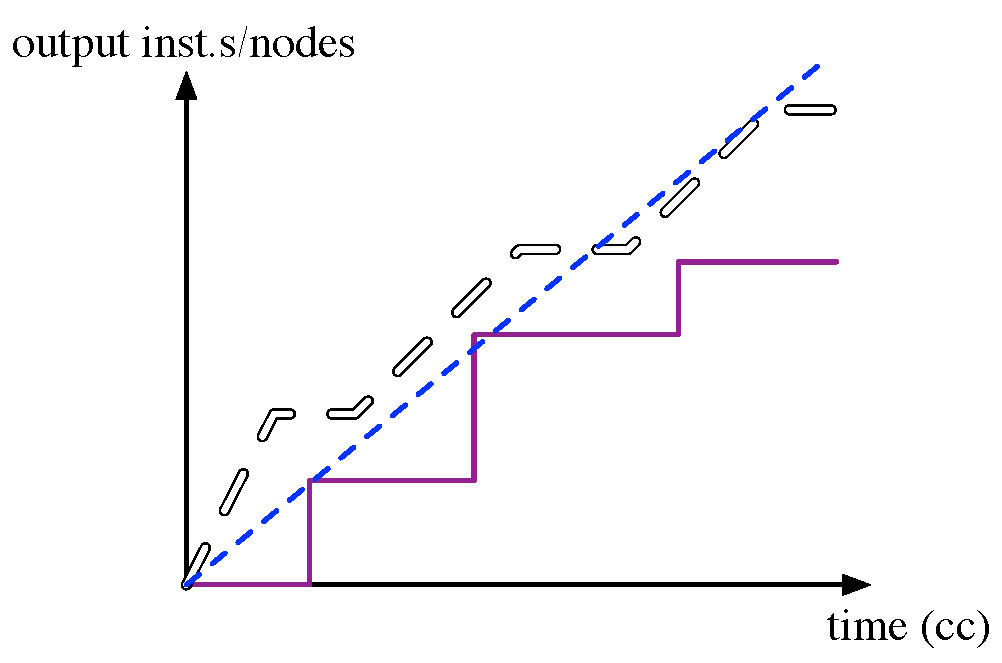
\includegraphics[width=\linewidth]{burstiness}
\caption{Burstiness}
\end{figure}

\subsection{Reconfiguration}
\subsection{Scheduling time}


\section{Experimental analysis}

\section{Conclusions and future work}

\bibliographystyle{IEEEtran}
\bibliography{../library/library}
\end{document}